\chapter{\label{ch:2-neutrinophysics}Neutrino Physics} 

%%%%%%%%%%%%%%%%%%%%%%%%%%%%%%%%%%%%%%%%%%%%%%%%%%%%%%%%%%%%%%%%%%%%%%%%%%%%%%%%
% From my COS report

% This chapter will cover details of relevant neutrino physics for the thesis 
% project. The theoretical aspects of neutrino physics will be reviewed 
% including the theory of neutrino oscillations in the PMNS framework. 
% Neutrino production will also be discussed including details of neutrino 
% production in supernovae and the role neutrinos can have in understanding 
% the mechanics of a supernova burst
 
% The work for this section is ongoing as it is associated with the analysis 
% work in the other sections, it is expected to be completed by the end of 
% December 2019.
%%%%%%%%%%%%%%%%%%%%%%%%%%%%%%%%%%%%%%%%%%%%%%%%%%%%%%%%%%%%%%%%%%%%%%%%%%%%%%%%

% TODO TODO TODO TODO TODO TODO TODO TODO TODO TODO TODO TODO TODO
% References
% Decide on historical vs theoretical overview or both
% TODO TODO TODO TODO TODO TODO TODO TODO TODO TODO TODO TODO TODO

% \minitoc

Despite being one of the most abundant particle in the universe, neutrinos are 
some of the most elusive; due to the fact that neutrinos can only interact via
the weak interaction. The history of neutrino physics is therefore strongly
connected to the discovery and study of weak interactions. Measurements by
Chadwick in 1914 showed that the energy spectrum of electrons released in
\(\beta\)--decays was continuous, this is in contrast to discrete spectra
observed in \(\alpha\) and \(\gamma\) decays, and seemingly violates
conservation of energy under the assumption of a two--body final state which was
expected at the time. In order to solve this problem, Pauli postulated that the
continuous energy spectrum could be explained if the energy released in a 
\(\beta\)--decay could be shared with an additional neutral weakly interacting 
fermion which Pauli named the neutron. Fermi later renamed Pauli's fermion to
the neutrino, after Chadwick discovered the neutron in 1932. Despite claims that
neutrinos might never be detected, neutrinos have now been discovered and they
have been found to have a number of interesting properties which were not
anticipated when neutrinos were first postulated. This chapter will detail some 
of the history and theory of neutrino's and their interactions.

In this chapter, Section \ref{nu_hist} will give a brief historical overview of 
neutrino physics, Section \ref{nu_osc} will introduce neutrino oscillations
and the theory used to describe them, while Section \ref{nu_prod} will discuss
neutrino interactions in matter as well as neutrino production. Finally Section
\ref{nu_sn} will discuss the production of neutrinos in supernovae, as well as
the role they could play in understanding supernovae.

\section{A Brief History of Neutrino Physics} \label{nu_hist}

The first attempt to incorporate the neutrino into a theoretical model came in
1934 when Fermi presented his theory of \(\beta\)--decay, in this theory the 
neutrino takes part in a four--point interaction with the other components of 
the \(\beta\)--decay interaction. The incredible success of this theory in
explaining the observed properties of \(\beta\)--decays provided strong evidence 
for the neutrinos existence, however, in 1934 after using Fermi's  theory to 
predict the strength of neutrino interactions, H. Bethe and R. Peierls found 
that the interactions were so weak that they might never be observed, a 
prediction that held true for over 20 years.

The first breakthrough in experimental neutrino physics would come in 1956. F.
Reines and C. Cowan were attempting to measure positrons produced in inverse 
\(\beta\)--decay interactions,
\begin{equation}
	\bar{\nu_e} + p \rightarrow n + e^+.
\end{equation}
A detector containing 1400 litres of liquid scintillator was used to measure the 
large flux of electron anti--neutrinos in the vicinity of the Savannah River 
nuclear reactor. They observed a large increase in the rate of positron events 
when the reactor was on when compared to when the reactor was switched off, the 
first experimental evidence for the existence of neutrinos. 

The discovery of the electron neutrino opened the door to answer questions of 
neutrino flavour. As neutrinos are produced alongside a charged lepton it is 
natural to compare the properties of neutrinos with their partners in the weak
interaction. At the time of the discovery of the neutrino there were two known
charged leptons, the electron and the muon, and so physicists asked whether the
neutrinos produced alongside muons are different from those produced alongside
electrons. In 1962, Lederman et al discovered the muon neutrino at Brookhaven
National Laboratory; by creating a beam of muon associated neutrinos using 
decaying pions, and observing the leptons produced in neutrino interactions 
after all other particles had been absorbed. They found that only muons where 
produced in the resulting neutrino interactions, and therefore the neutrinos 
produced were only ever associated with a muon, which shows that neutrinos are 
produced with a distinct flavour in weak interactions.

With the discovery of the tau--lepton in 1977 it was expected that there should 
be an associated tau neutrino, however, it wouldn't be detected until 2001 by 
the DONUT experiment. In the experiment, tau neutrinos where produced from the
decay of charmed mesons produced in collisions between protons and a stationary
target. The neutrino interactions where detected in emulsion detectors, where
the unique geometry of the interaction, in which a short tau track is produced
at the vertex followed by a long muon track, allowed them to be distinguished 
from other decays.

While additional neutrino species are possible, data from measurements of the Z 
boson line--shape at LEP in 1992 restricts the number of active light neutrino 
species to be three. An active light neutrino is any neutrino with \(m_\nu <
\frac{m_Z}{2}\) that can interact with the Z boson, such that the decay \(Z 
\rightarrow \nu \nu \) is possible.

Alongside the discovery of three different types of neutrino, there were
interesting results when observing neutrinos produced in the Sun. The flux of
neutrinos from the Sun at the earth surface had been predicted with Bachall's 
Standard Solar Mode, however, in 1968 when Davis et al measured the flux in the
Homestake experiment they found a deficit with respect to the prediction of the
standard solar model (SSM) \cite{TODO}, the so called solar neutrino problem. In 
the Homestake experiment electron neutrinos where being measured via there 
inverse beta decay interactions with the chlorine in the target,
\begin{equation}
	v_e + ^{37}\mbox{Cl} \rightarrow ^{37}\mbox{Ar} + e^-.
\end{equation}
The neutrino interaction rate was measured by counting the number of argon 
atoms in the chlorine tank by capturing them on helium gas which was
periodically bubbled through the chamber.

In addition to the solar neutrino problem, a similar deficit was observed in
1988 for muon neutrinos produced during cosmic ray showers in the atmosphere.
The Kamiokande experiment was able to measure both electron and muon neutrino 
interactions via the cerenkov radiation produced by the charged leptons in 
water, their data was consistent with the expected rate of electron neutrinos 
from the atmosphere, however, a deficit of muon neutrinos was observed. 

The next generation of the Kamiokande experiment, Super Kamiokande, aimed to
understand the observed deficit of atmospheric muon neutrinos with a larger 
water cerenkov detector capable of resolving the angular distribution of 
atmospheric neutrino interactions. Super Kamiokande consists of a cylindrical 
vessel containing 50kt of ultra pure water, surrounded by an array of around 13
,000 photomultiplier tubes to detect the cerenkov light. Electron and muon 
neutrinos can be distinguished based on the pattern of cerenkov light that is 
left in the detector; due to their higher mass muons leave clear cerenkov 
rings in the detector while electrons, which can scatter and shower, tend to 
leave diffuse "fuzzy" rings on the wall of the detector. In 1998, Super 
Kamiokande published measurements of the flux of atmospheric muon neutrinos as 
a function of azimuthal angle. Since these neutrinos are created a short 
distance from the earths surface, the incoming angle of the neutrino can be 
used to estimate the distance travelled by the neutrino before arriving at the 
detector; the down--going neutrinos have only travelled a short distance in 
the atmosphere (\(\sim 10\mbox{km}\)), while the up--going neutrinos have 
travelled through the entire earth to reach the detector (\(\sim 13,000\mbox{km
}\)). Figure \ref{fig:sk_flux}, shows the flux of neutrinos measured by Super 
Kamiokande as a function of distance travelled; the muon neutrino flux is 
consistent with the no oscillation prediction at small \(\mbox{L} / \mbox{E}_\
nu\), however, for large \(\mbox{L} / \mbox{E}_\nu\) a clear deficit is 
observed. 

\begin{figure}

	\centering

	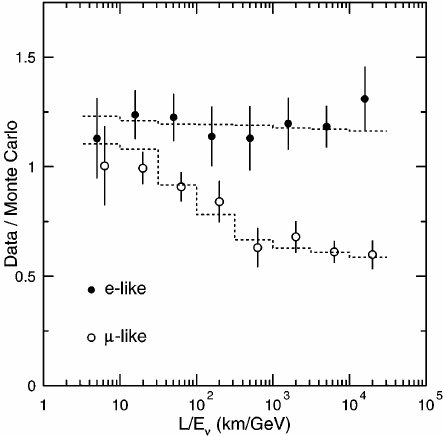
\includegraphics[width=0.7\textwidth]{figures/sk_flux.jpg}

	\caption
	[Ratio of data to Monte Carlo for electron and muon neutrino fluxes 
	measured by the Super Kamiokande experiment as a function of 
	\(\mbox{L} / \mbox{E}_\nu\).]
	{Ratio of data to Monte Carlo for electron and muon neutrino fluxes measured 
	by the Super Kamiokande experiment as a function of 
	\(\mbox{L} / \mbox{E}_\nu\). The Monte Carlo prediction is based on the
	assumption of no oscillations. The muon neutrino flux is consistent with the
	no oscillation prediction at small \(\mbox{L} / \mbox{E}_\nu\), however, for
	large \(\mbox{L} / \mbox{E}_\nu\) a clear deficit is observed. The best fit
	under the assumption of atmospheric (\(\nu_\mu \rightarrow \nu_\tau\))
	oscillations is shown, the best fit parameters are \(\Delta m^2 = 2.2 \times
	10^{-3} \mbox{eV}^2\), and \(sin^22\theta = 1\) \cite{Fukuda1998}.}

	\label{fig:sk_flux}

\end{figure}

While it wouldn't completely solve the solar neutrino problem, the Sudbury
Neutrino Observatory (SNO) was able to provide unique insight into the observed
solar neutrino fluxes in 2002. Unlike other water cerenkov detectors, SNO 
was filled with heavy water, \(\mbox{D}_2\mbox{O}\), instead of its lighter 
isotope. The use of heavy water in the detector gives rise to additional 
neutrino interactions which allowed the SNO experiment to distinguish between 
three different interaction modes: charged current (CC), neutral current (NC), 
and elastic scattering (ES). Each interaction mode is sensitive to different 
parts of the solar neutrino flux, including some sensitivity to the muon 
neutrino and tau neutrino fluxes via the NC and ES interactions. Analysis of the 
data for each of the three unique interaction modes lead to a measurement of 
the flavour composition of the solar neutrino flux at earth, while also 
measuring an overall neutrino flux at earth that is consistent with the SSM.
Figure \ref{fig:sno_flux} shows the composition of the solar neutrino flux as 
measured in the SNO experiment \cite{Ahmad2002}, the flux prediction based on 
the measured rate of NC events is consistent with the predictions of the 
SSM. The composition of solar neutrinos measured in the SNO experiment was not
a result of neutrino oscillations, instead it is the result of matter effects on
the neutrino propagation via the Mikheyev–Smirnov–Wolfenstein (MSW) effect.

\begin{figure}

	\centering

	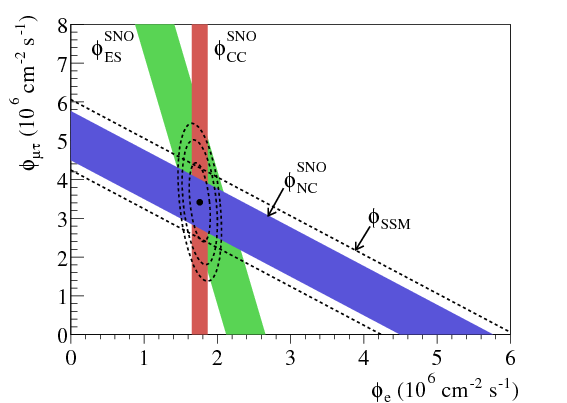
\includegraphics[width=0.8\textwidth]{figures/sno_flux.png}

	\caption
	[Solar neutrino flux composition as measured by the SNO experiment.]
	{Solar neutrino flux composition as measured by the SNO experiment. The
	coloured bands represent the measured flux of charged current (CC),
	neutral current (NC), and elastic scattering (ES) events, including a \(\pm 1
	\sigma\) spread. The central contours represent 68\%, 95\%, and 99\%
	probability contours for the joint \(\phi_e\) and \(\phi_{\mu \tau}\) fit. The
	dashed lines represent the predicted flux of \(^8\mbox{B}\) neutrinos based on 
	the standard solar model \cite{Ahmad2002}. }

	\label{fig:sno_flux}

\end{figure}

After the results of the SNO experiment there were still a number of possible
solutions to the solar neutrino problem \cite{Smirnov2016}; TODO. In order for
neutrino oscillations to be the unique solution to the problem, an
\(\mbox{L/E}_\nu\) dependence would have to be measured. To make this
measurement a much shorter neutrino baseline would be needed, along with a
source of neutrinos with a small energy spread, and a detector with good energy
resolution. In 2002 the Kamioka Liquid Scintillator Anti--neutrino Detector
(KamLAND) experiment measured \(\bar{\nu_e}\) oscillations from a number of
nuclear reactors with an average baseline of 180km. Along with an overall
deficit of neutrino events, they were able to use the high energy resolution of
the KamLAND detector to measure an \(\mbox{L/E}_\nu\) dependence of the 
\(\bar{\nu_e}\) survival probability. Figure \ref{fig:kamland_spectrum},
shows the ratio of the observed neutrino flux with the no oscillation predicted
flux as a function of \(\mbox{L/E}_\nu\), a clear dependence can be seen and
this data was enough to make neutrino oscillations the unique solution to the
solar neutrino problem.

\begin{figure}

	\centering

	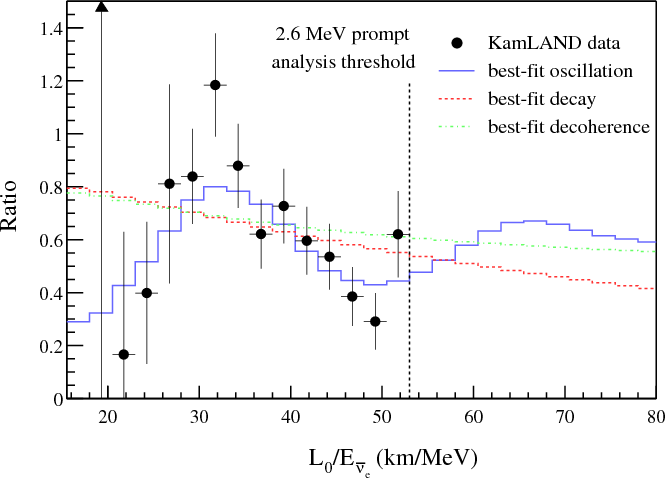
\includegraphics[width=0.8\textwidth]{figures/kamland_spec.png}

	\caption
	[Ratio of observed neutrino flux to the predicted flux in the absence of
	neutrino oscillations in the KamLAND experiment.]
	{Ratio of observed neutrino flux to the predicted flux in the absence of
	neutrino oscillations in the KamLAND experiment.}

	\label{fig:kamland_spectrum}

\end{figure}

Since the discovery of neutrino oscillations, ...

%%%%%%%%%%%%%%%%%%%%%%%%%%%%%%%%%%%%%%%%%%%%%%%%%%%%%%%%%%%%%%%%%%%%%%%%%%%%%%%%
% TODO
% Neutral Current & gargamelle
% Opera
% precision with daya bay etc.
%%%%%%%%%%%%%%%%%%%%%%%%%%%%%%%%%%%%%%%%%%%%%%%%%%%%%%%%%%%%%%%%%%%%%%%%%%%%%%%%

% \section{Neutrinos in the Standard Model} \label{nu_sm}

\section{Neutrino Oscillations} \label{nu_osc}

\section{Neutrino Interactions} \label{nu_prod}

\section{Supernova Neutrinos} \label{nu_sn}
